%************************************************
\section{The Agent} % (fold)
\label{sec:impl_the_agent}
%************************************************
As described in Section \ref{sec:the_agent}, the Agent component enables the simulation user to control the virtual agent in order to move around and interact with the environment. Moreover, it triggers the classification event and the interaction callback methods on the EgocentricApp. The agent component implements three components presented in the design \ref{fig:final_architecture}: First Person Agent, Agent Control Trigger and Classification Trigger.\\

The First Person Agent component is implemented as a standalone class, having at its core the Camera and ActionListener classes from the JME3 core library. Figure \ref{fig:impl_first_person_agent} depicts the class diagram of the first person agent.
\begin{figure}[H]
	\centering
	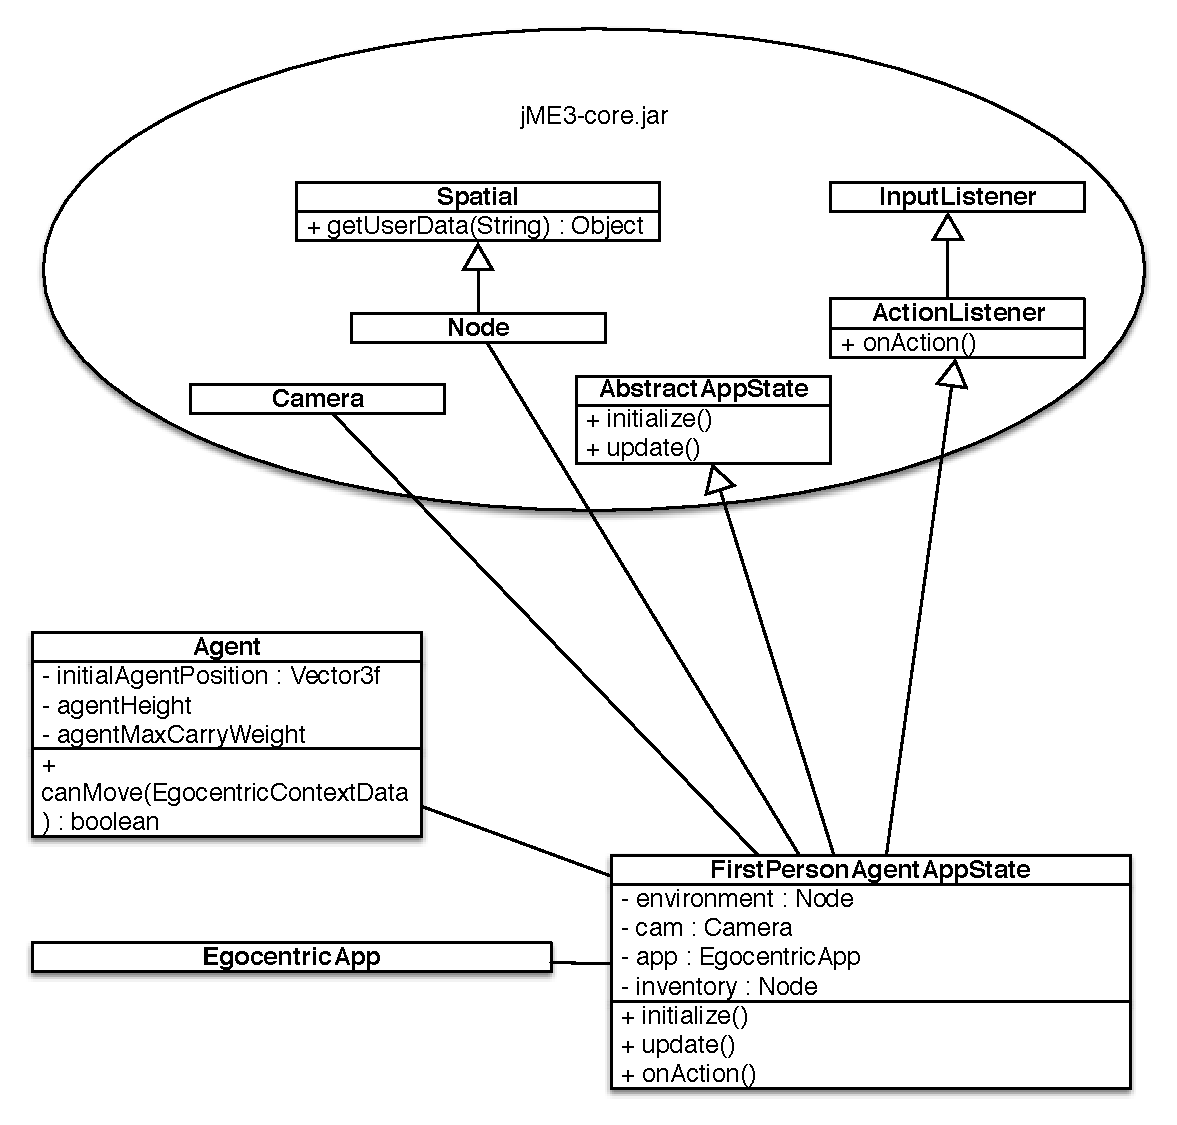
\includegraphics[width=\linewidth]{gfx/Chapter4/first_person_agent}
	\caption{First Person Agent Class Diagram}
	\label{fig:impl_first_person_agent}
\end{figure}

To implement the requirements for the agent \ref{us:4}, we have isolated the implementation in concrete AbstractAppState, which is a jME3 abstraction that allows you to control the global game logic and the overall game mechanics. This allows to create a modular implementation of the framework, instead of having all the game logic related functionality implemented in the EgocentricApp. Just like SimpleApplication, AbstractAppState provides an initialization method which is called once, after the scene graph has been initialized and an update method, which is called on every render step of the rendering engine. The number of render steps of the rendering engine is measured in Frames Per Second (FPS) and it depends on each machines graphical processing capabilities.\\

%************************************************
\subsection{First Person Agent} % (fold)
\label{subsec:impl_the_first_agent}
%************************************************
The first person agent is a wrapper around the Camera which is placed within the rendered 3D environment. The camera is initially positioned at the initialAgentPosition and height given by the Agent class. Also, agentMaxCarryWeight is worth mentioning -- this has impact when the agent tries to pick up an object, which is possible if the object's weight is less or equal to agentMaxCarryWeight.\\

To help targeting objects, we have placed a cross sign in the middle of the screen which is always visible. Figure \ref{fig:impl_crosshair} depicts a screen shot of the agent targeting the Pot object on the Stove with the help of the on-screen CrossHair.
\begin{figure}[H]
	\centering
	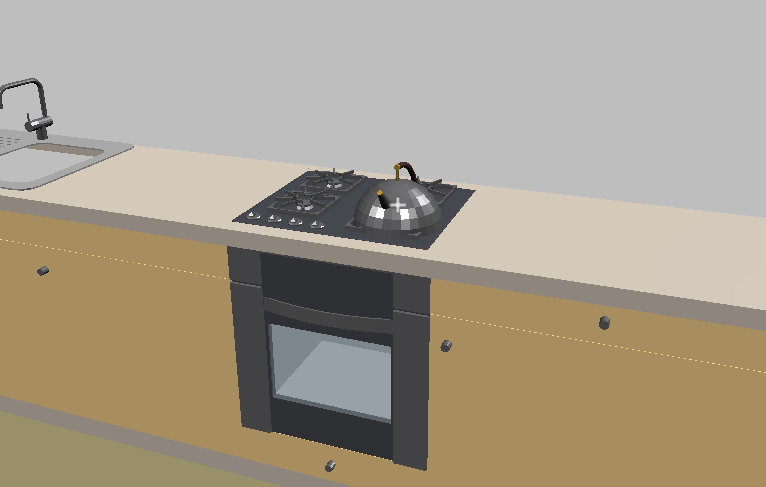
\includegraphics[width=0.8\linewidth]{gfx/Chapter4/aiming}
	\caption{A cross hair always visible in the middle of the screen to help targeting objects}
	\label{fig:impl_crosshair}
\end{figure}

To represent picked-up objects, we have implemented an inventory. As illustrated in Figure \ref{fig:impl_inventory}, the inventory is a miniature representation of the picked up object and mover around together with the agent.\\
\begin{figure}[H]
	\centering
	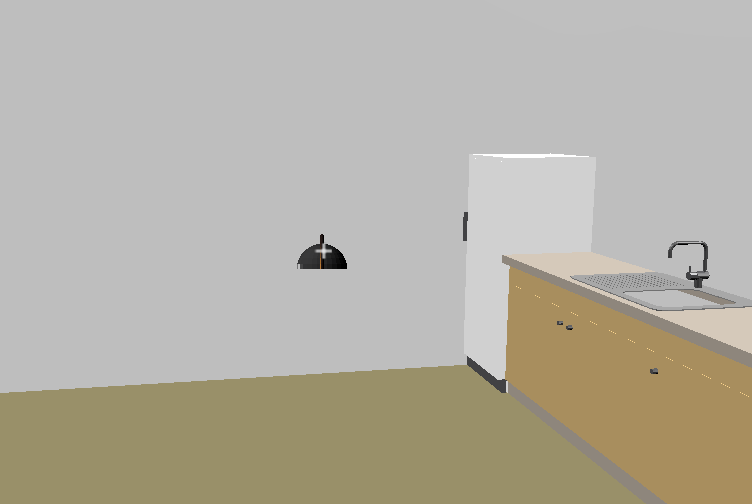
\includegraphics[width=0.8\linewidth]{gfx/Chapter4/inventory}
	\caption{Representation of a picked up object}
	\label{fig:impl_inventory}
\end{figure}

To allow the game engine to automatically handle collision between the agent and the rendered 3D environment, we have used a the CharacterControl entity from the core library. The control contains a cylinder shape which is placed at the initial agent position and is moved together with the agent. This shape entity is not visually rendered. The character control together with the collision control component the scene was wrapped in by the simulation runtime, prevent the agent from passing through the rigid areas of the environment (walls, objects, etc).\\

Controlling the agent and interacting with the environment is detailed in Section \ref{subsec:sd_controlling_the_agent} of the user guide.
% section impl_the_first_agent (end)

%************************************************
\subsection{Agent Control Trigger} % (fold)
\label{subsec:impl_agent_control}
%************************************************
By implementing the ActionListener interface from the JME core library, we receive onAction() callbacks from the game engine whenever an input event is triggered (e.g. the mouse is moved, a key on the keyboard is pressed, etc). In the onAction() method we are listening for key presses (W, A, S, D), mouse movements and mouse clicks (left click, right click).\\

As already mentioned before, the view the agent has is represented by the Camera which is positioned within the 3D environment by means of a location vector and direction vector. The key presses influence the location of the camera, while the mouse movements influence the its direction.\\

When the left mouse button is clicked, it triggers an interaction event with the environment. To determine the object the agent tries to interact with, we cast a ray of infinite length from the camera's current position along the it's direction. We intersect this ray with the \emph{environmentScene} stored in the EgocentricApp singleton. The intersection results in a lost of Spatials which intersected with the ray. We sort this list by proximity and get the closes Spatial, which is the first object displayed on screen pointed at by the cross hair. Next, if the spatial doesn't carry EgocentricContextData, the action is dismissed and warning message is displayed on screen (''Interaction possible only with egocentric entities''). Otherwise, we retrieve the EgocentricContextData as \emph{contextData} and the adequate action is taken based on the current context. The context based decision flow can be analysed in the source code going through the FirstPersonAgentAppState.interactListener.\\
% section impl_agent_control (end)

%************************************************
\subsection{Classification Trigger} % (fold)
\label{subsec:impl_classification_trigger}
%************************************************
To start the classification process on the monitoring service, we have implemented another ActionListener, where we listen for any action that can change the field of vision of the agent. That is key presses (W, A, S, D) and mouse movements. If any of these actions is carried out, we trigger a new classification on the Monitoring Service \ref{sec:impl_monitoring_service}.
% section impl_classification_trigger (end)

% section impl_the_agent (end)